%% beamerthemeImperialPoster v1.0 2016/10/01
%% Beamer poster theme created for Imperial College by LianTze Lim (Overleaf)
%% LICENSE: LPPL 1.3
%%
%% This is the example poster demonstrating use
%% of the Imperial College Beamer Poster Theme
\documentclass[xcolor={table}]{beamer}
%% Possible paper sizes: a0, a0b, a1, a2, a3, a4 (although Imperial College posters are usually A0 or A1).
%% Possible orientations: portrait, landscape
%% Font sizes can be changed using the scale option.
\usepackage[size=a0,orientation=portrait,scale=1.55]{beamerposter}
\usepackage{amsmath}
\usetheme{ImperialPoster}
\usepackage{shorts}
\usepackage{lipsum}
% \usepackage{babel}
\usepackage{subfigure}
\usepackage{graphicx}
\usepackage[ampersand]{easylist}
%% Four available colour themes
\usecolortheme{ImperialWhite} % Default
\title{{\large Machine learning continuously monitored systems: parameter estimation and beyond}}

\author{ {\normalsize Matías Bilkis, Giulio Gasbarri and John Calsamiglia  - Universitat Autònoma de Barcelona}}

\institute{}%Física Teòrica: Informació i Fenòmens Quàntics, Departament de Física,

\addbibresource{sample.bib}


\begin{document}
\begin{frame}[fragile=singleslide,t]\centering

\maketitle

\begin{columns}[onlytextwidth,T]

%%%% First Column
\begin{column}{.47\textwidth}

\begin{block}{Abstract}
  \parshape 1 0cm \dimexpr\linewidth-0cm\relax
  We consider the problem of estimating parameters that govern the dynamics of a continuously monitored system. To this purpose, we bring into stage the machine-learning-machinery, allowing us to do maximum likelihood over the measurement signal, and compare its performance with respect Lorenztian fits of the spectral power and the Fisher information. We next move on to machine-learning-estimate parameters governing the dynamics of external controls, leaving doors and questions open to whether our approach can in turn be useful to tackle more sophisticated tasks, such as the identification of dynamical equations of motion out of measurement data.
\end{block}

\begin{block}{The model}
  \parshape 1 0cm \dimexpr\linewidth-0cm\relax
We consider an optomechanical system under continuous homodyne detection on the optical mode, in the Gaussian regime. The equations of motion read:
\begin{align}\label{eq:evo}
dx_t &= \big(A_\theta - \chi(\Sigma_t) C\big) x_t dt + \chi(\Sigma_t) dy = A_\theta x_t dt + \chi(\Sigma_t) dW_t \\
d\Sigma_t &= A_\theta \Sigma_t + \Sigma A_\theta^T + D - \chi(\Sigma_t)^T \chi(\Sigma_t) \nonumber¸\\
dy &= C(x_tdt + C^{-1}dW_t), \nonumber
\end{align}
where $(x_t,\Sigma_t)$ are the first two moments of the mechanical mode at time $t$, and $dy_t$ denotes measurement outcome; thus the measurement model is Gaussian centered on the value of the \textit{hidden} state $x_t$. Below we show a realization of the process; among all coefficients $\theta$ and matrices governing the dynamics, we here focus on $A_\theta$, which in the case of a damped oscillator reads {\small$A_{\theta} = \Big(\begin{matrix}-\gamma& -\omega\\\omega & -\gamma\end{matrix}\Big)$}.

{\center
  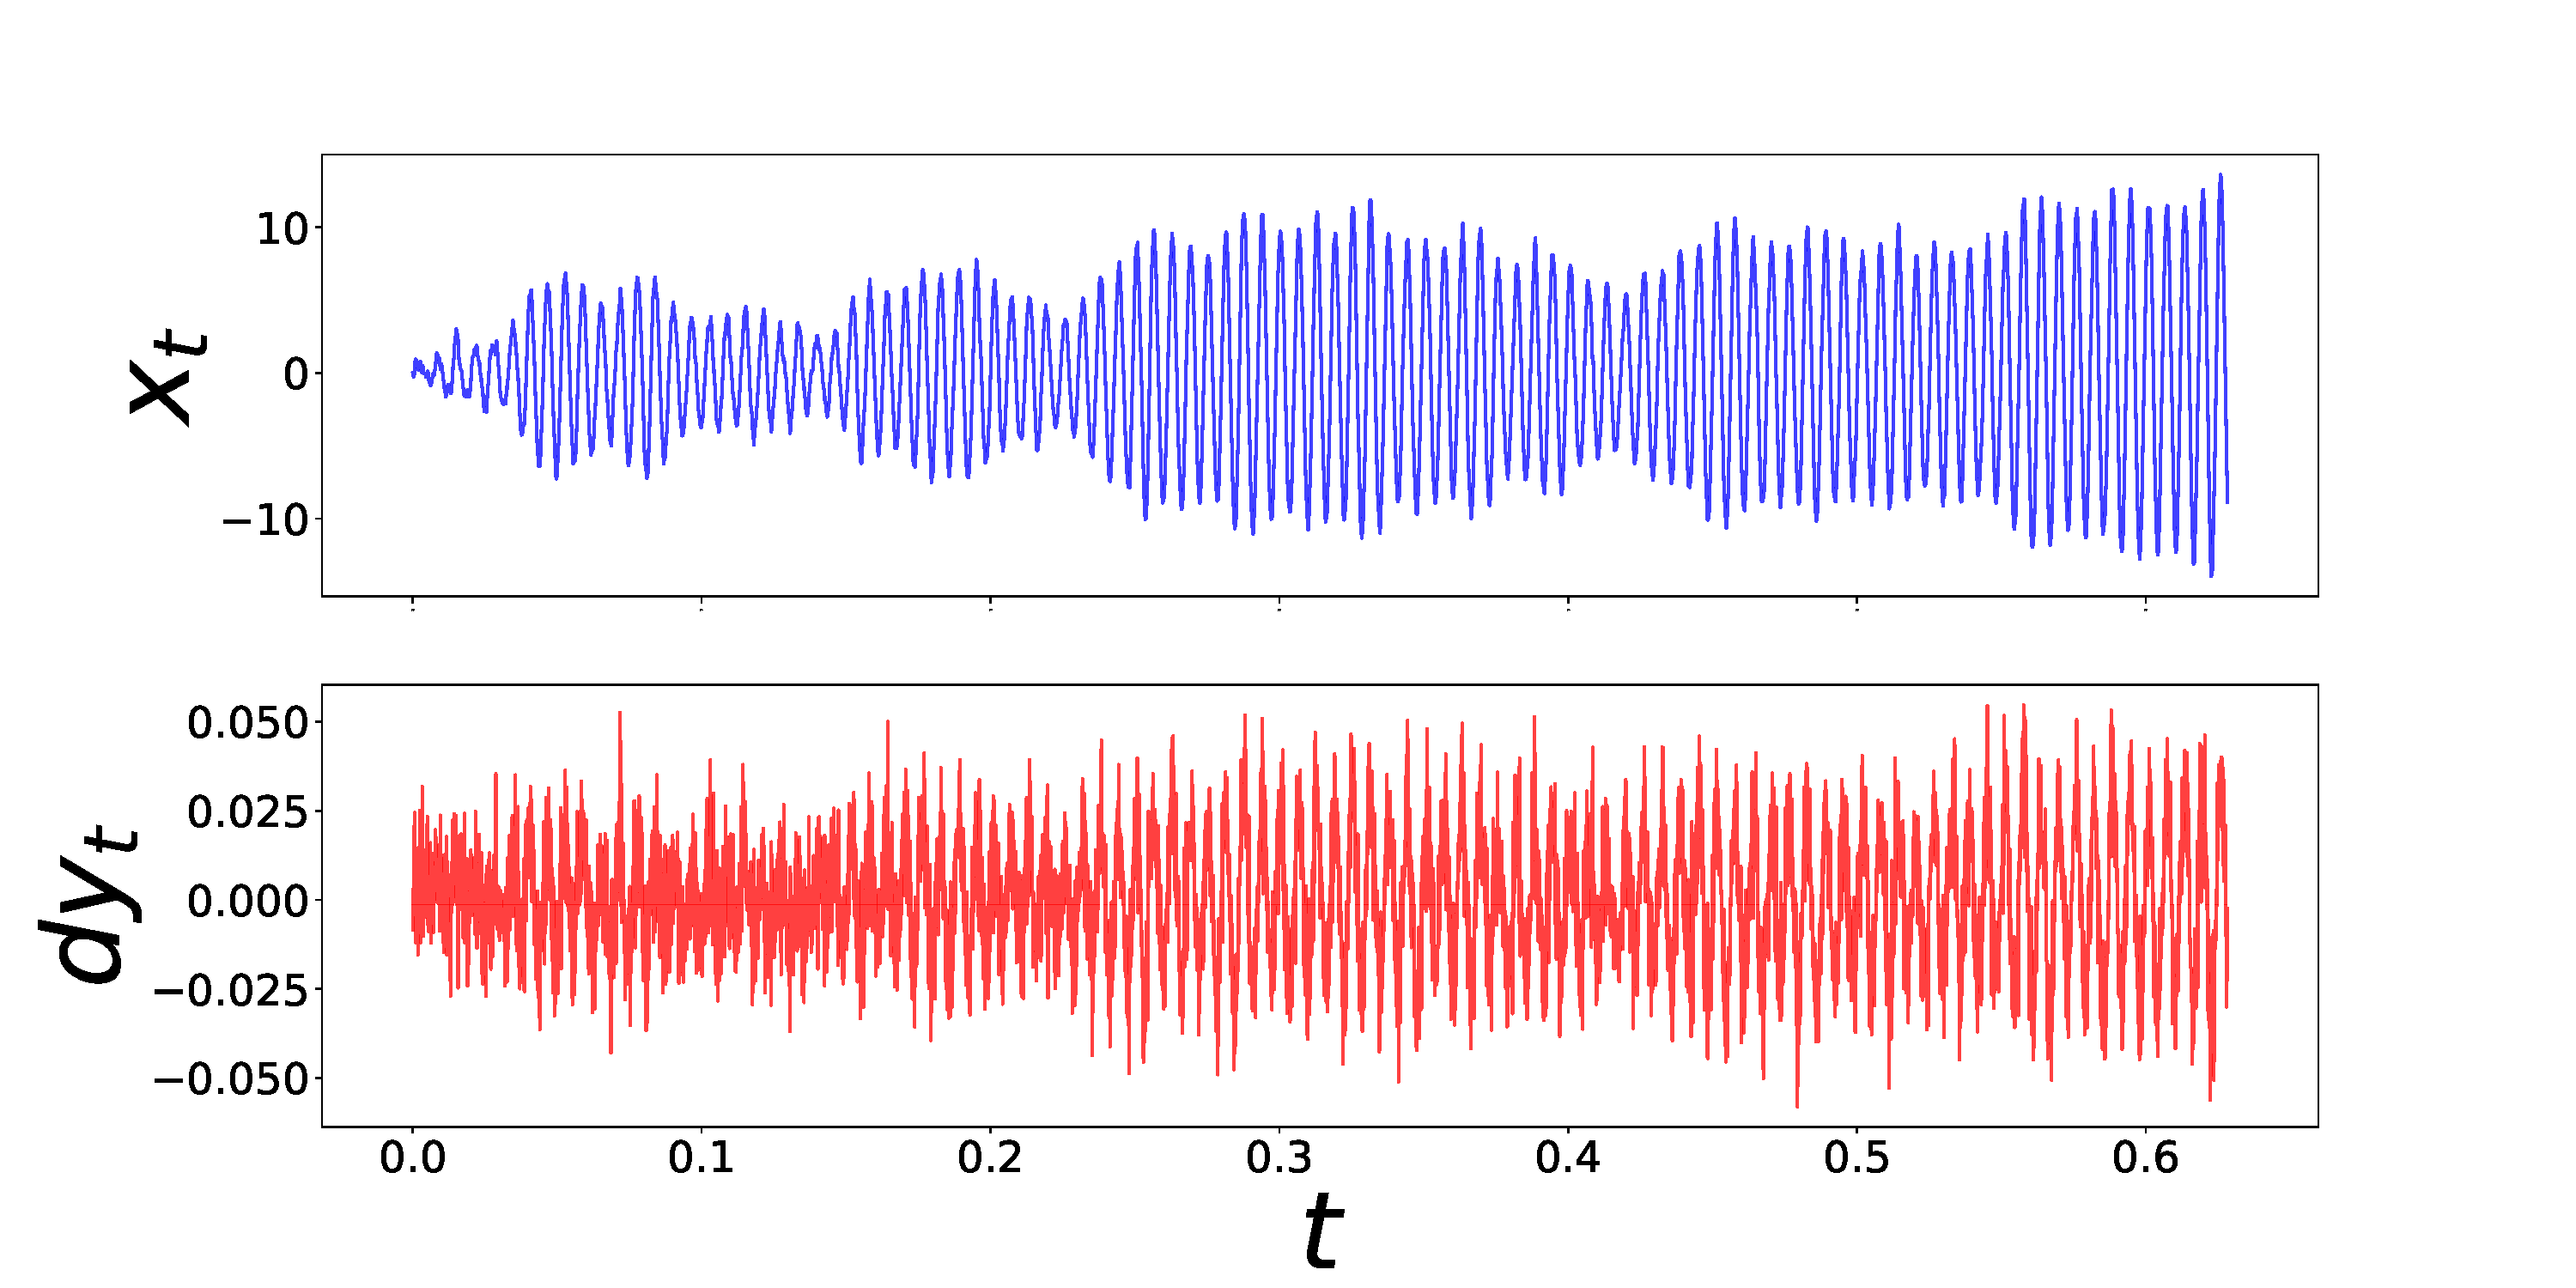
\includegraphics[width=.45\hsize]{figures_poster/evolution.pdf}
  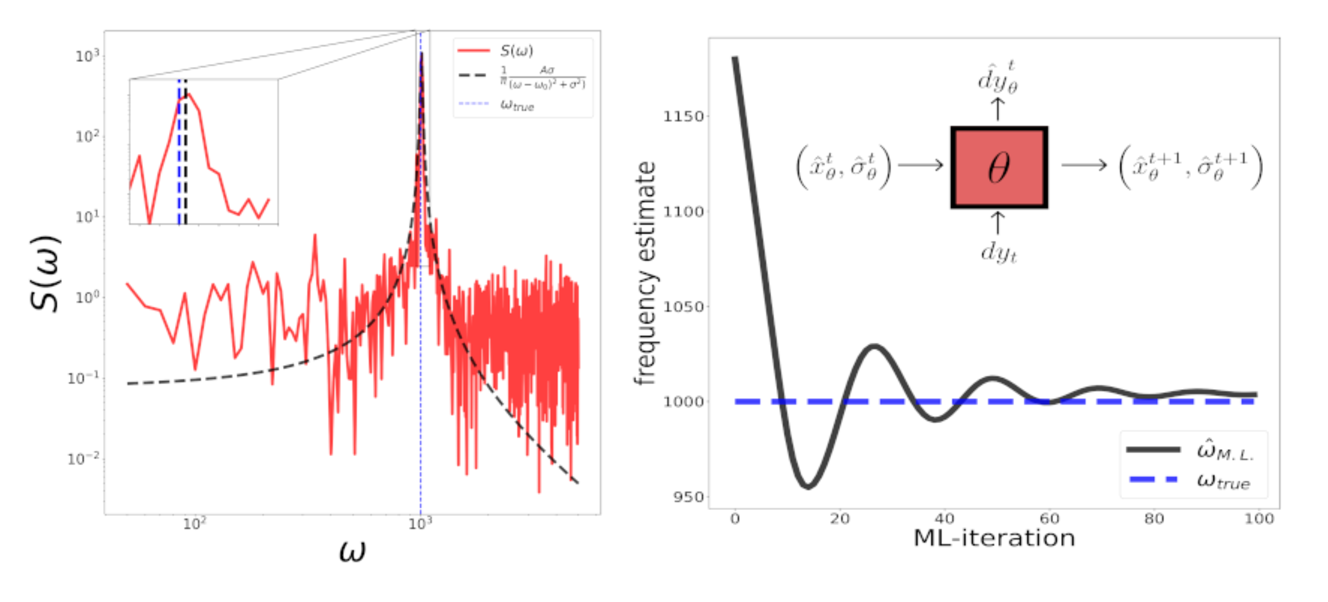
\includegraphics[width=.5\hsize]{figures_poster/dos.pdf}}
\end{block}

\begin{block}{Estimation}
  \parshape 1 0cm \dimexpr\linewidth-0cm\relax
  The log-likelihood $\lambda(y|\theta) = \log p(y|\theta)$ of getting a string of outcomes $y= (dy_0, ... dy_t)$ under parameter $\theta$ can be computed through the measurement model, and in particular the evolution of the score $\partial_\theta \lambda(y|\theta)$ can be derived, which permits to numerically integrate the Fisher information $I[\theta]$. This quantity lower bounds the variance of any unbiased estimation $\hat{\theta}$. Here, we propose a recurrent unit which computes $\hat{\theta} = \text{argmax}\lambda(y|\hat{x}_{\hat{\theta}})$ where $\hat{x}_{\hat{\theta}}$
  \textit{tracks} the hidden state in ressemblance to the Kalman Filter. We compare this estimation  $\hat{\omega}$ with traditional Lorentzian fit over the spectral power, and the Cramer-Rao bound.
{\center
    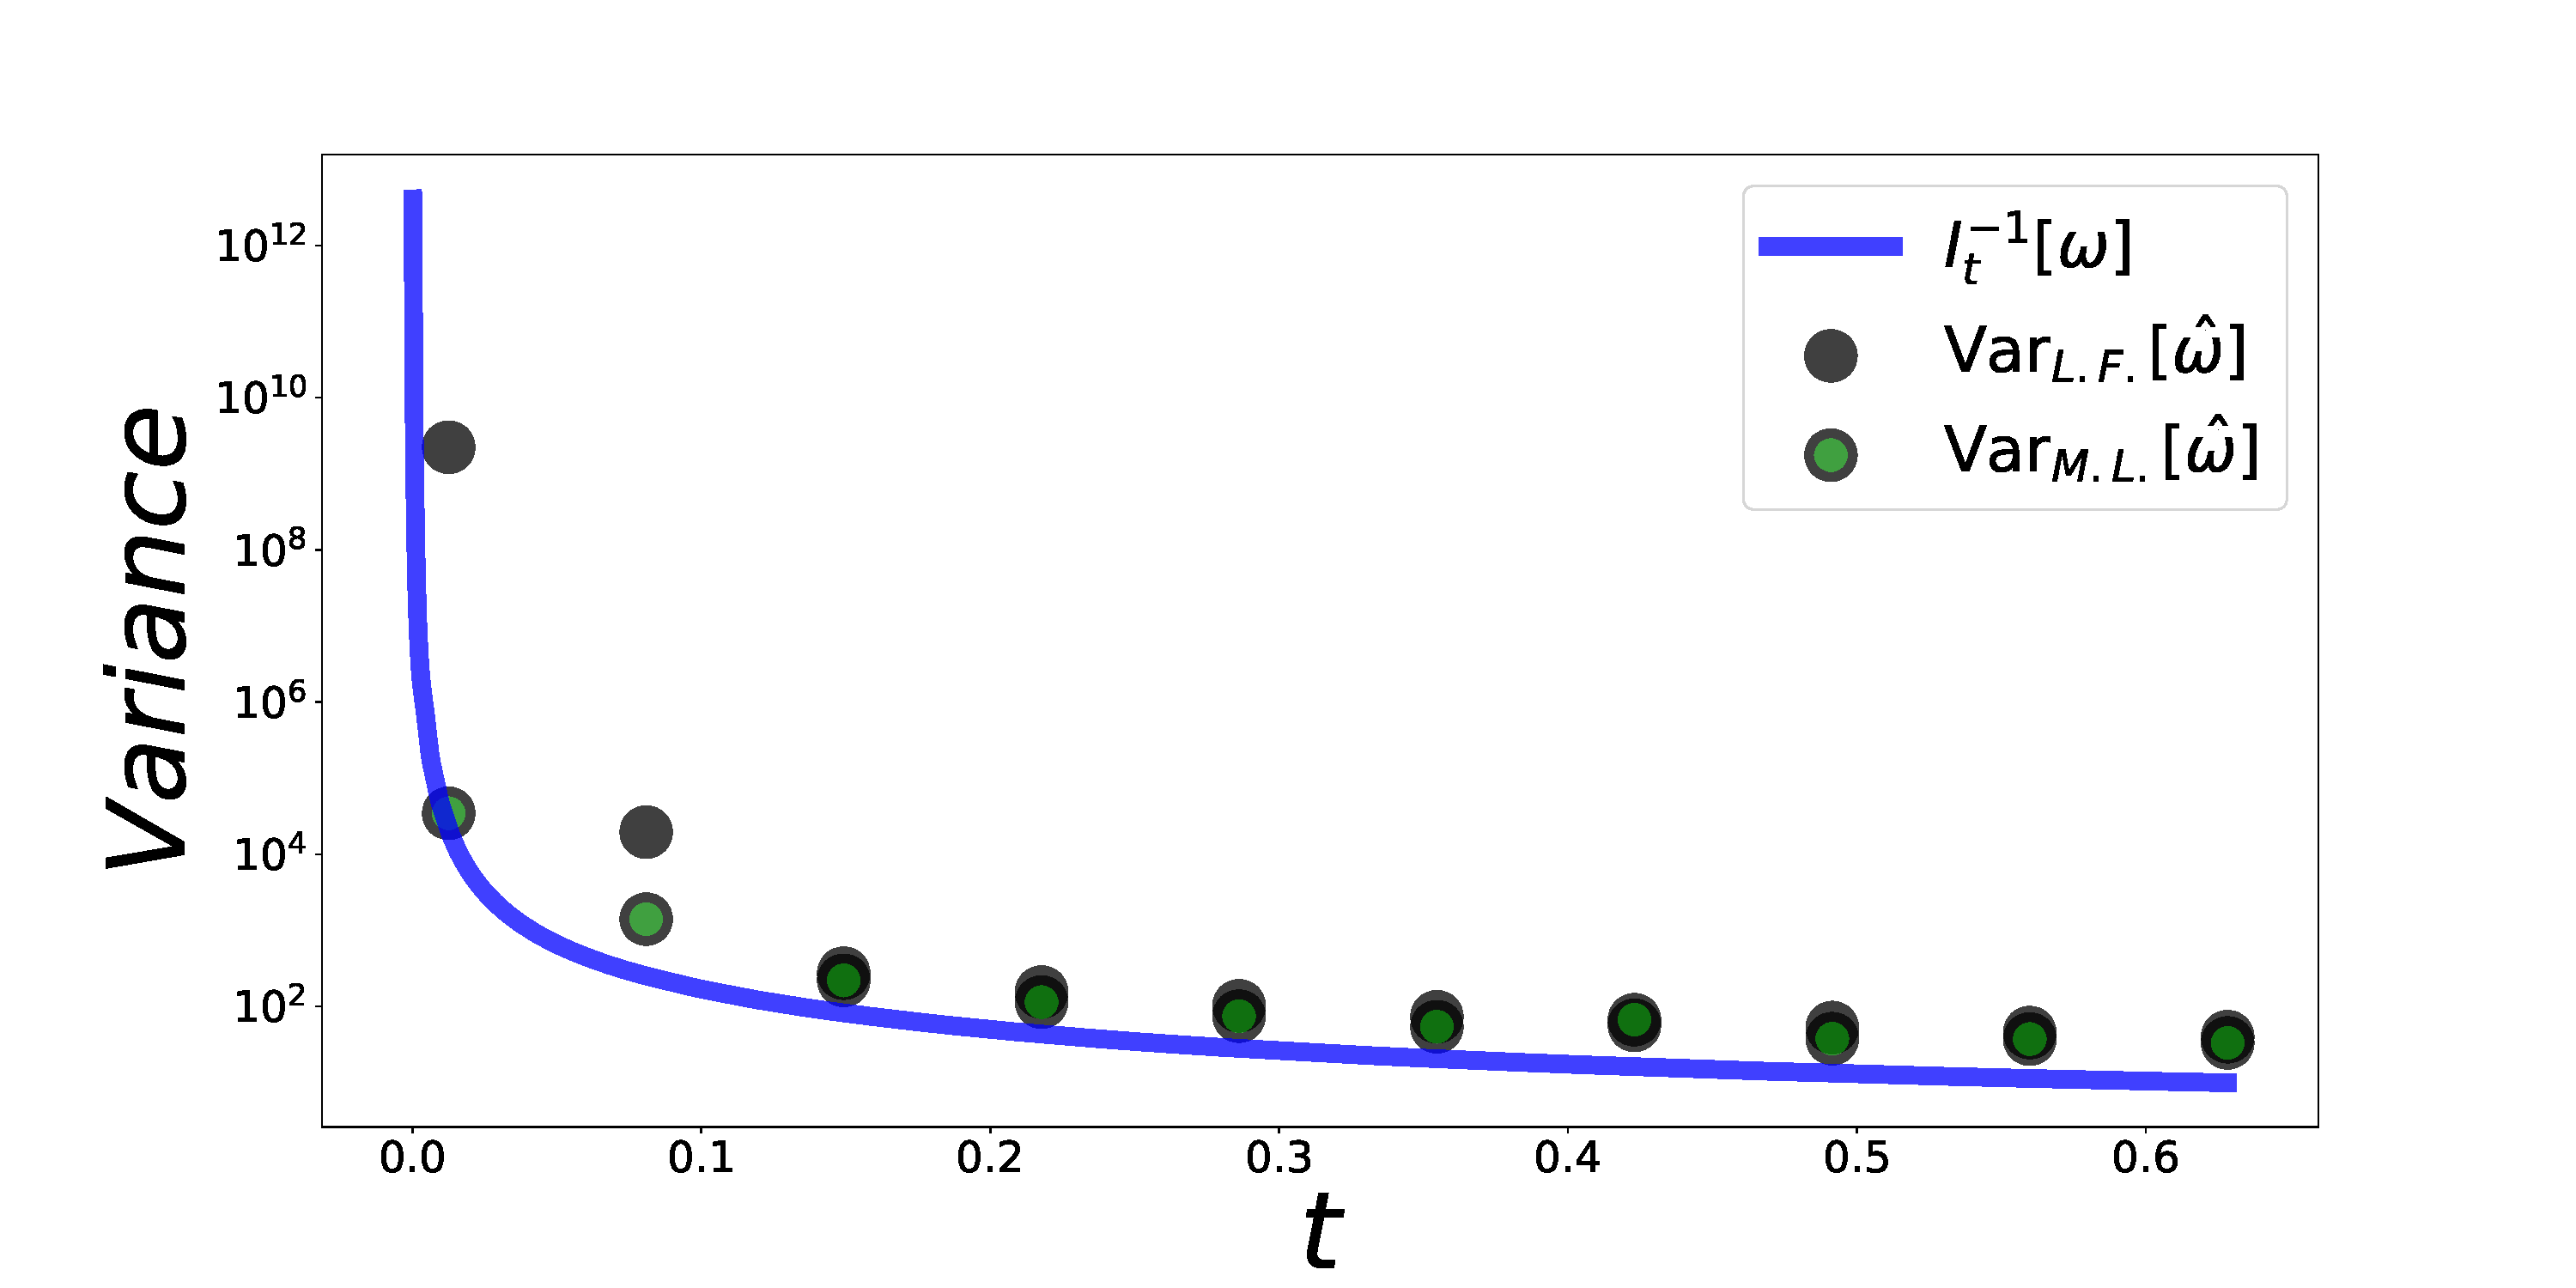
\includegraphics[width=1.\hsize]{figures_poster/variance_comparison_hori.pdf}
}
\end{block}
\end{column}

%%%% Second Column
\begin{column}{.47\textwidth}
\begin{block}{External controls}
  Signals $f^t_\theta$ can be included in the evolution ~\eqref{eq:evo} as:
  \begin{align}
  dx_t &= \big(A_\theta - \chi(\Sigma_t) C\big) x_t dt + \chi(\Sigma_t) dy + f^t_\theta dt
  \end{align}
  While the structure of the signal might potentially be complicated, we test our machine-learning machinery under the case of \textit{(i)} constant force, \textit{e.g.} $f^t_\theta = f$ , and \textit{(ii)} eponentially damped force  \textit{e.g.} $f^t_\theta = A e^{-t/\tau}$. Here, the task is to estimate $f$ and $(A, \tau)$ respectively out of measurement signal $dy_t$.
{\center
  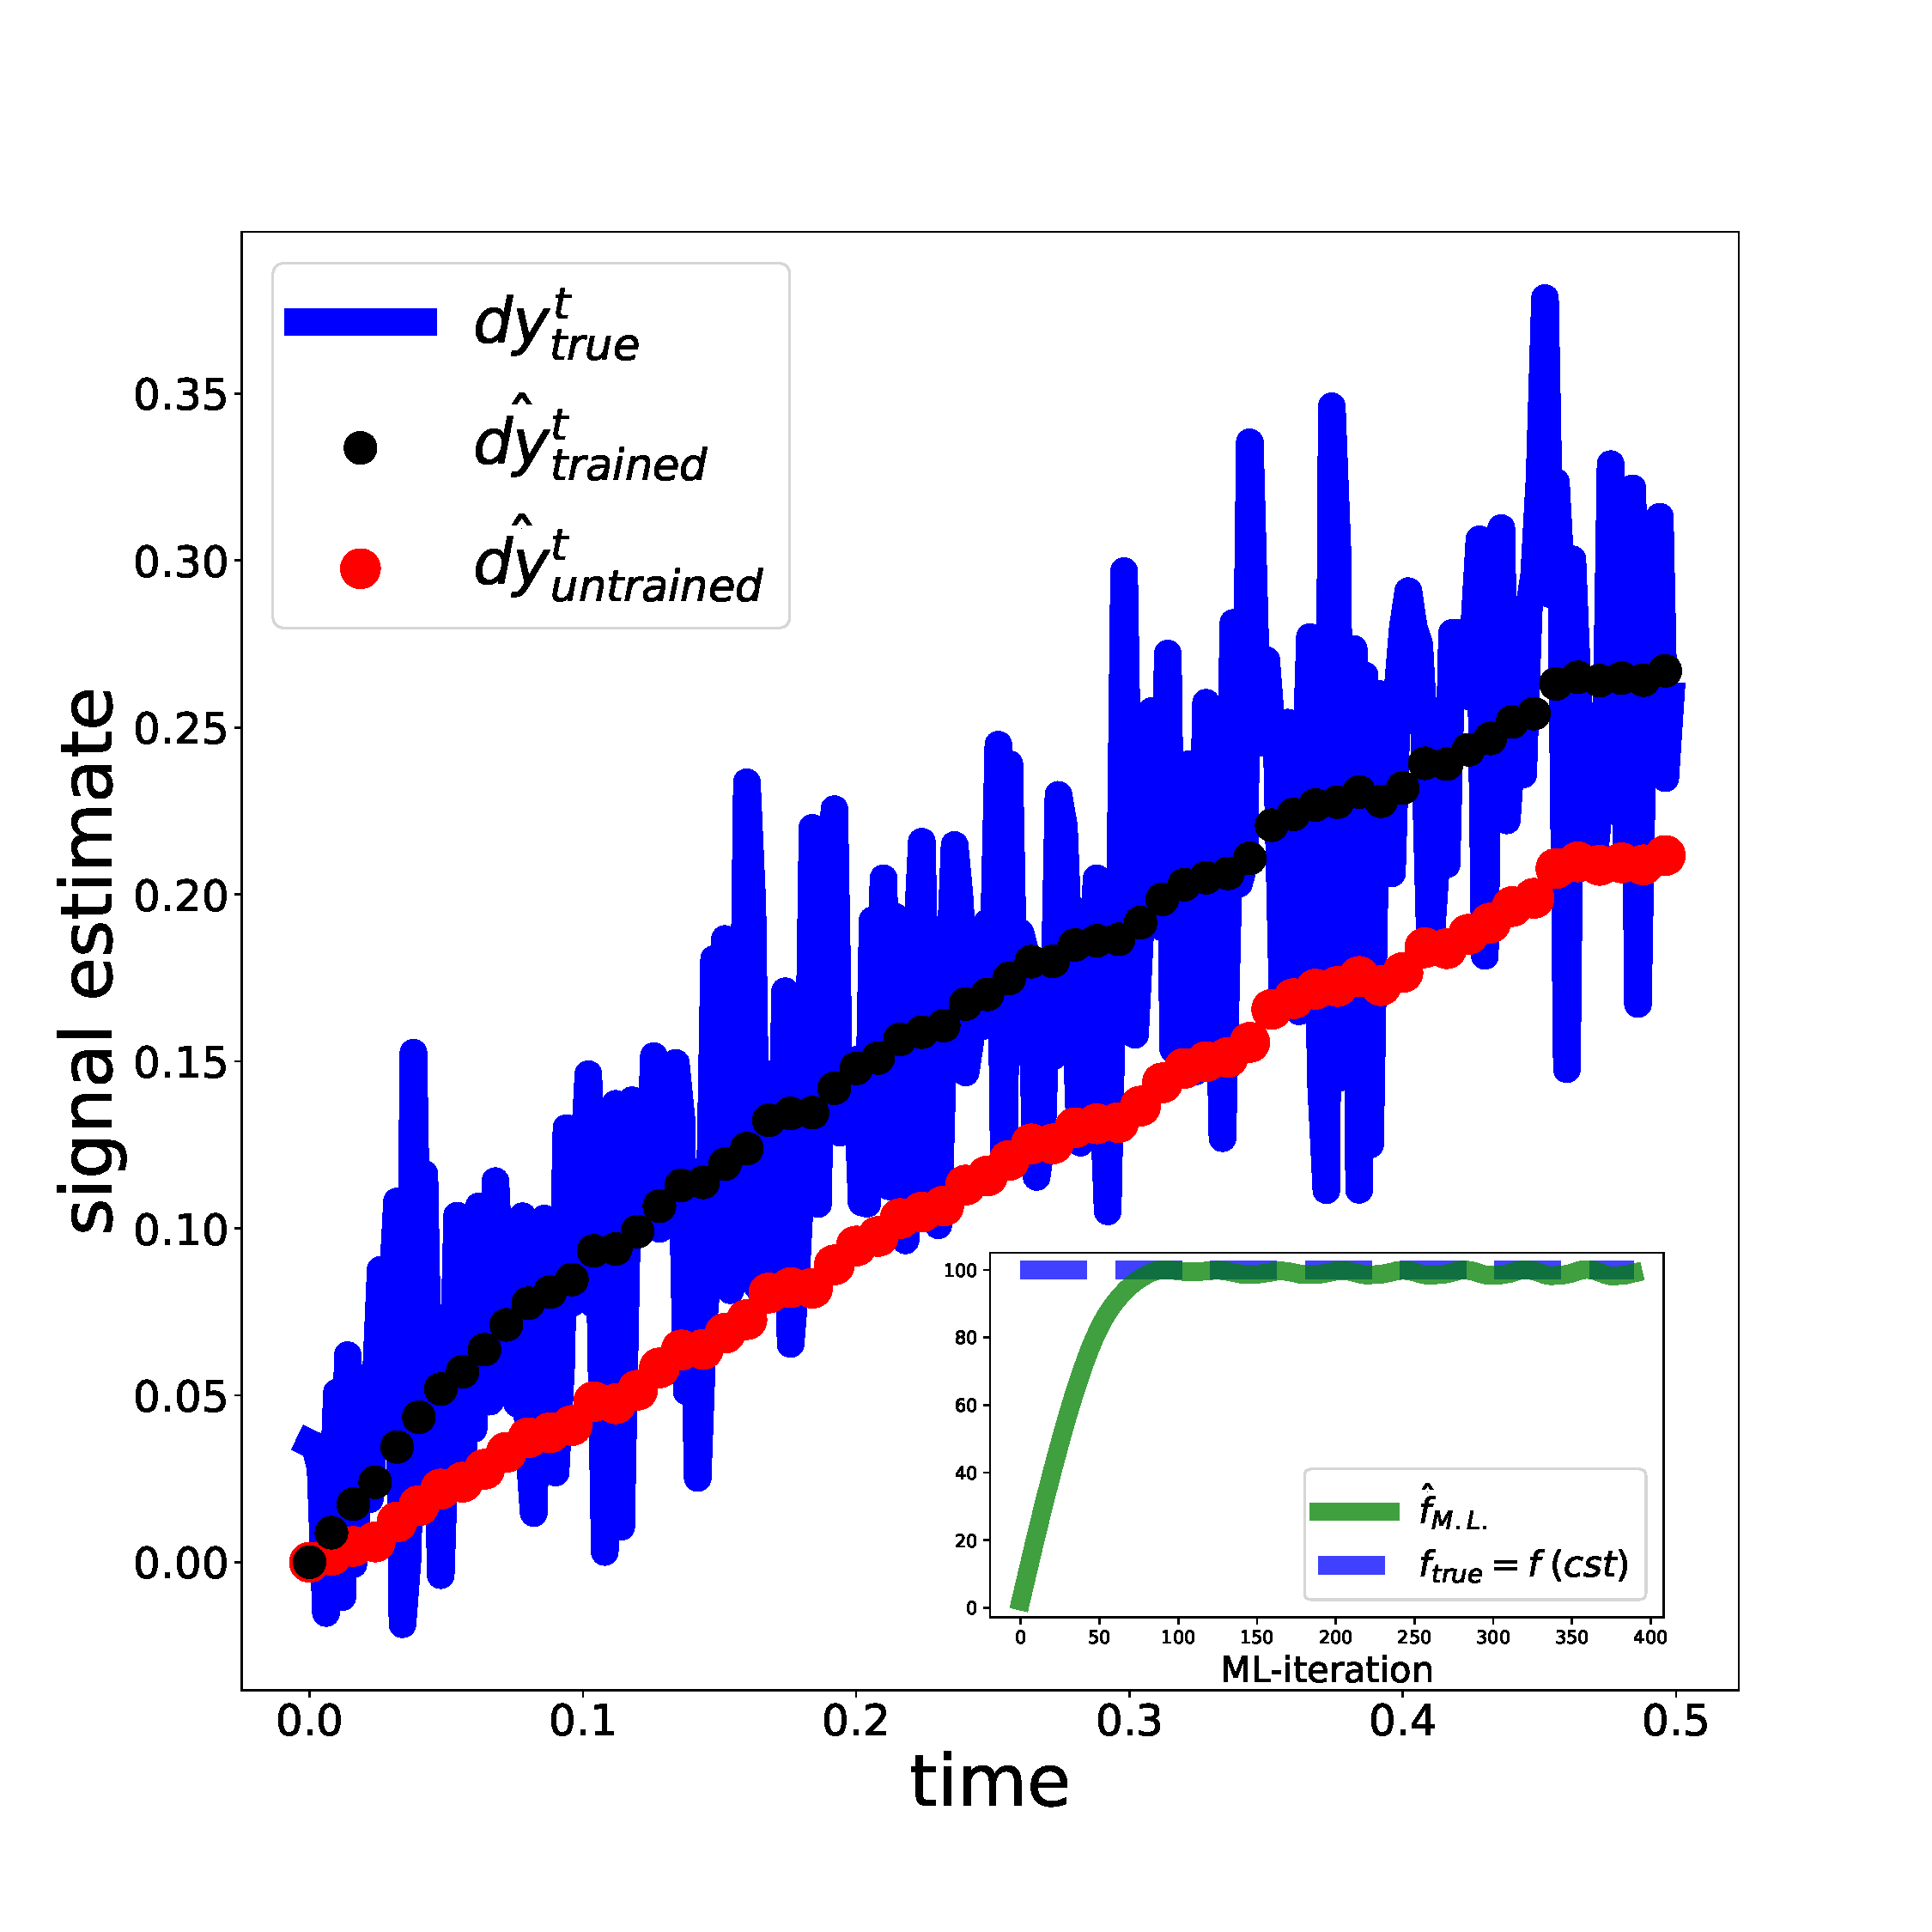
\includegraphics[width=.9\textwidth]{figures_poster/external_learn_signals.pdf}
  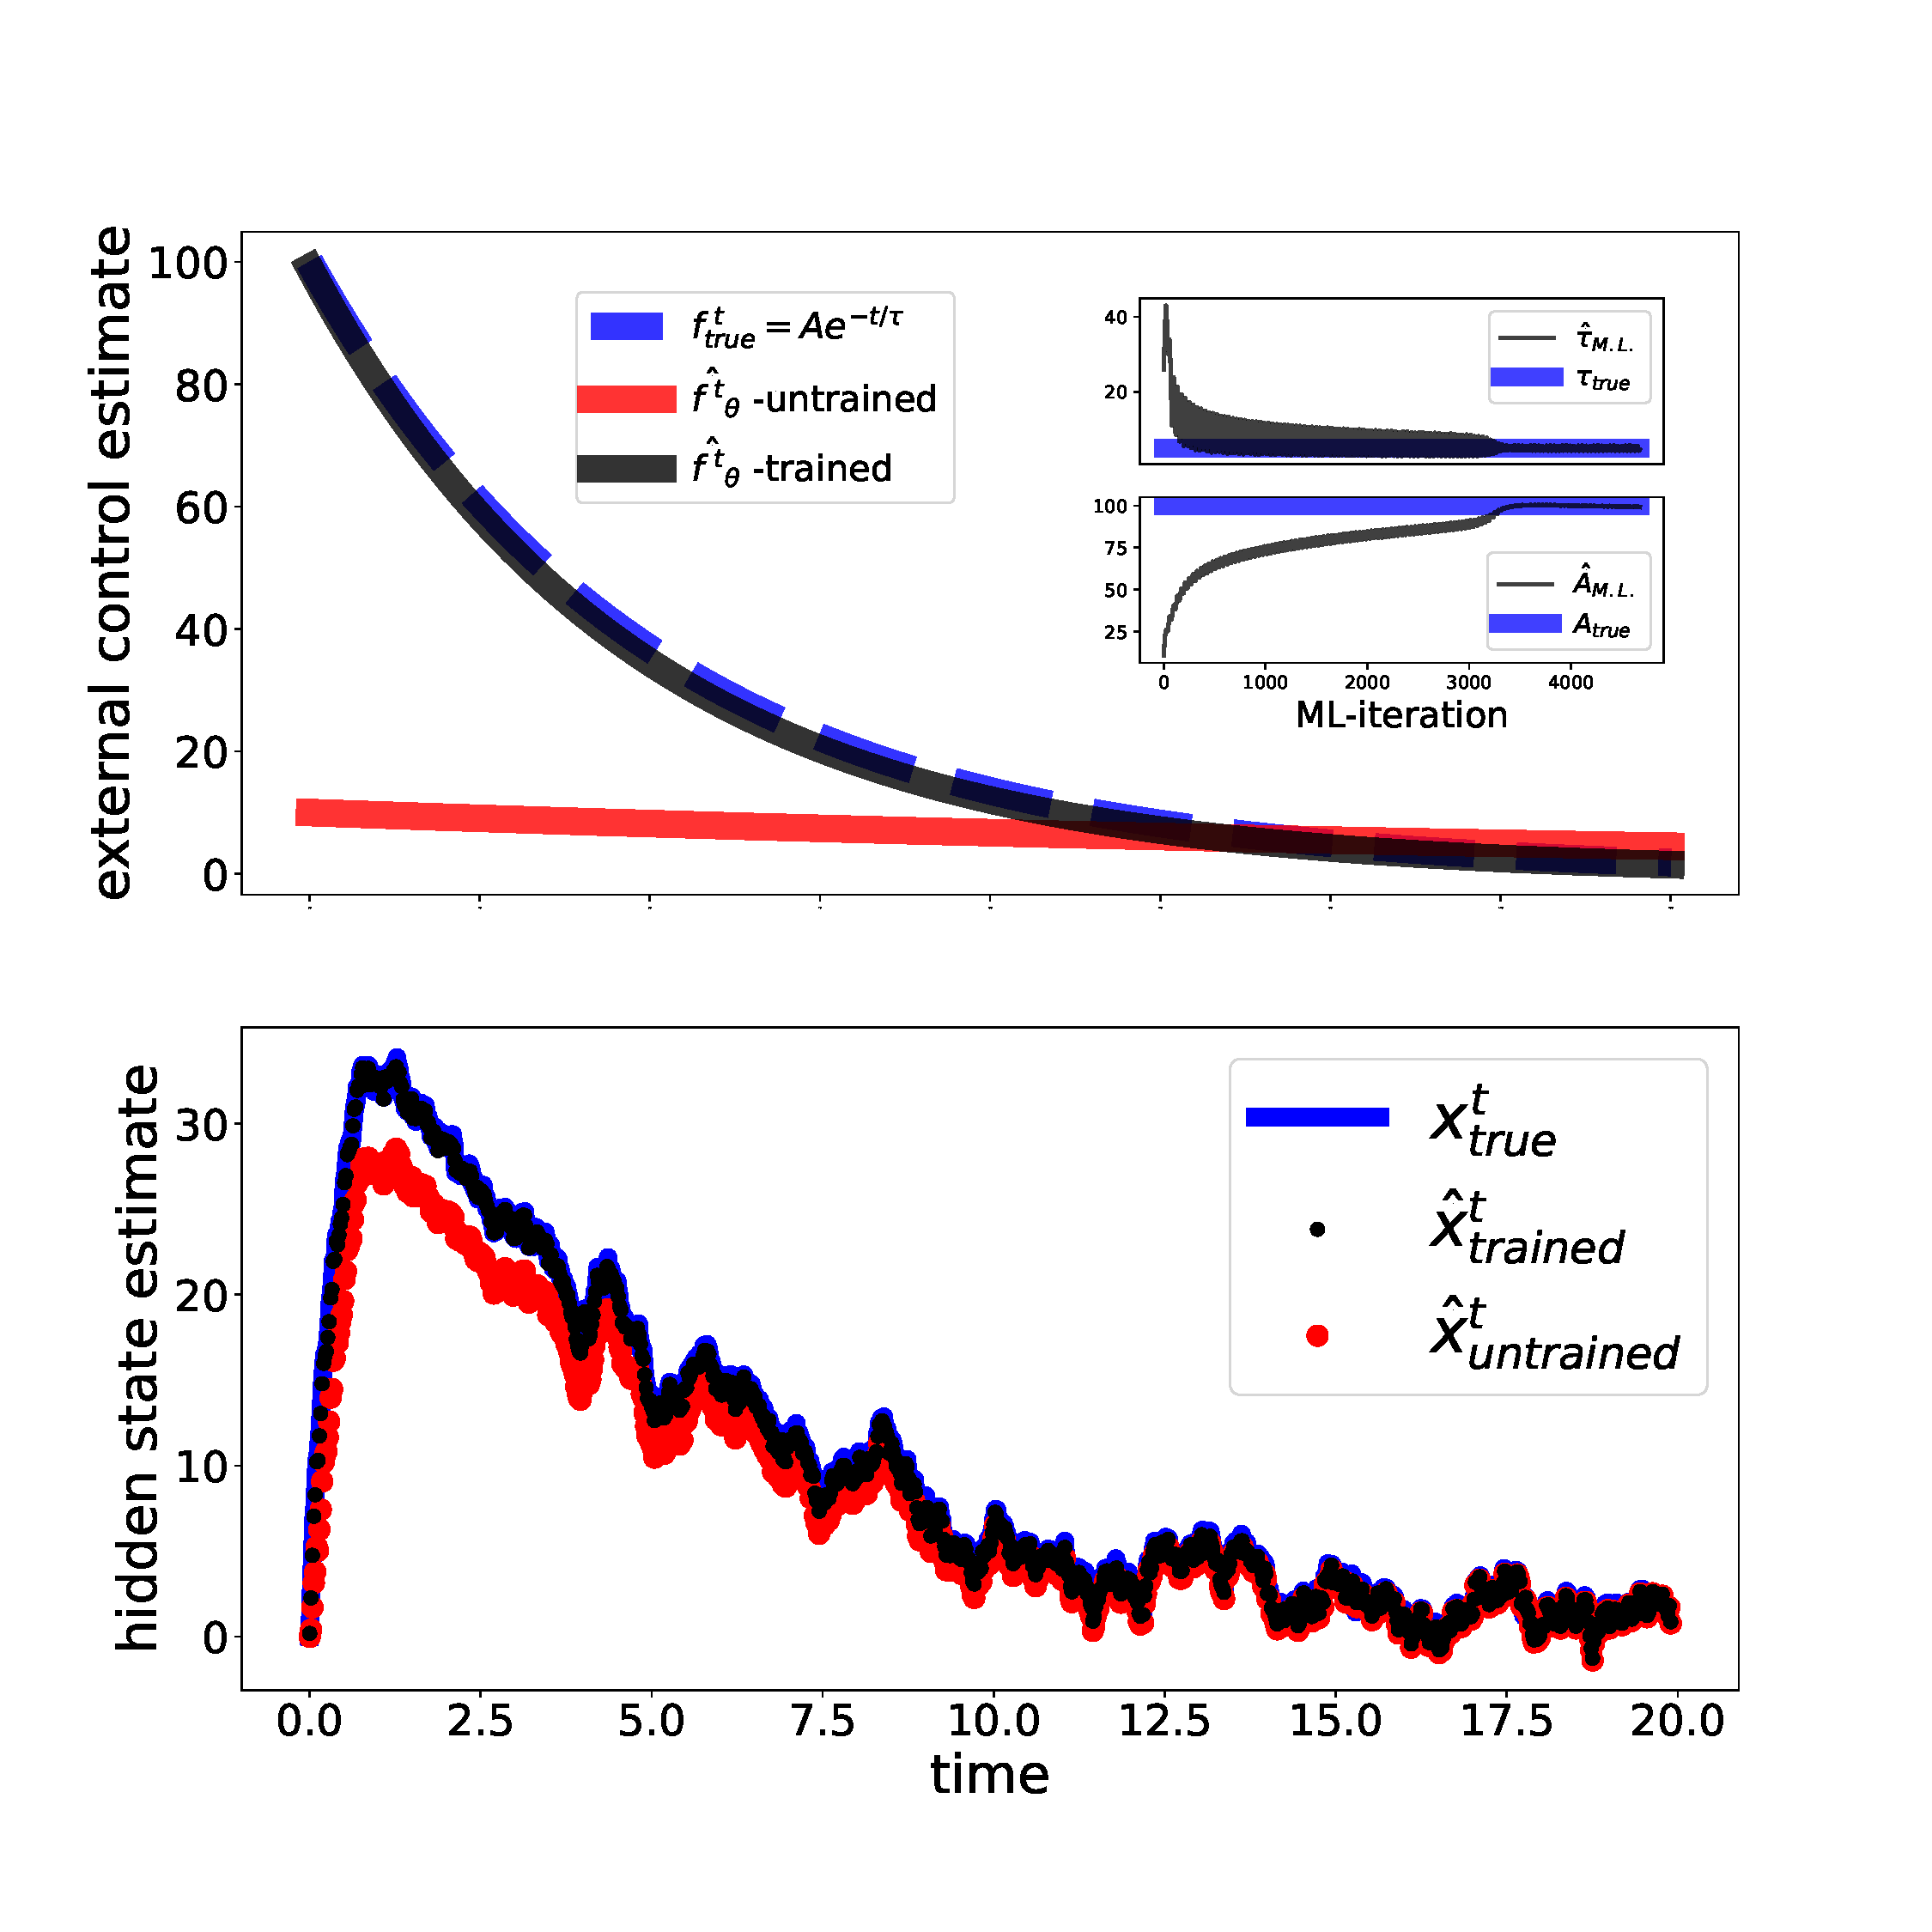
\includegraphics[width=.9\textwidth]{figures_poster/external_learn_track_example2.pdf}
  }
\end{block}


\begin{block}{Conclusion}
  We introduced a machine-learning method, i.e. a recurrent cell which (aided with automatic differentiator methods) is able to track and estimate the dynamics of a hidden Markov system. Among interesting directions are those of inferring dynamical equations out of measurement data, in cases where $f_\theta^t$ has a more sophisticated structure.
  \end{block}


\begin{block}{Code}

\includegraphics[width=.15\textwidth]{figures_poster/qr_repo.pdf}
\end{block}


\printbibliography

\end{column}
\end{columns}


\end{frame}
\end{document}
